\documentclass{article}

\usepackage{charter} % Use the Charter font

\usepackage[
	a4paper,    % Paper size
	top=1in,    % Top margin
	bottom=1in, % Bottom margin
	left=1in,   % Left margin
	right=1in,  % Right margin
	%showframe  % Uncomment to show frames around the margins for debugging purposes
]{geometry}

\setlength{\parindent}{0pt}     % Paragraph indentation 
\setlength{\parskip}{1em}       % Vertical space between paragraphs

\usepackage{graphicx}       % Required for including images

\usepackage{fancyhdr}       % Required for customizing headers and footers

\fancypagestyle{firstpage}{%
	\fancyhf{} % Clear default headers/footers
	\renewcommand{\headrulewidth}{0pt} % No header rule
	\renewcommand{\footrulewidth}{1pt} % Footer rule thickness
}

\fancypagestyle{subsequentpages}{%
	\fancyhf{} % Clear default headers/footers
	\renewcommand{\headrulewidth}{1pt} % Header rule thickness
	\renewcommand{\footrulewidth}{1pt} % Footer rule thickness
}

\AtBeginDocument{\thispagestyle{firstpage}} % Use the first page headers/footers style on the first page
\pagestyle{subsequentpages} % Use the subsequent pages headers/footers style on subsequent pages

%----------------------------------------------------------------------------------------

\begin{document}

%----------------------------------------------------------------------------------------
%	FIRST PAGE HEADER
%----------------------------------------------------------------------------------------

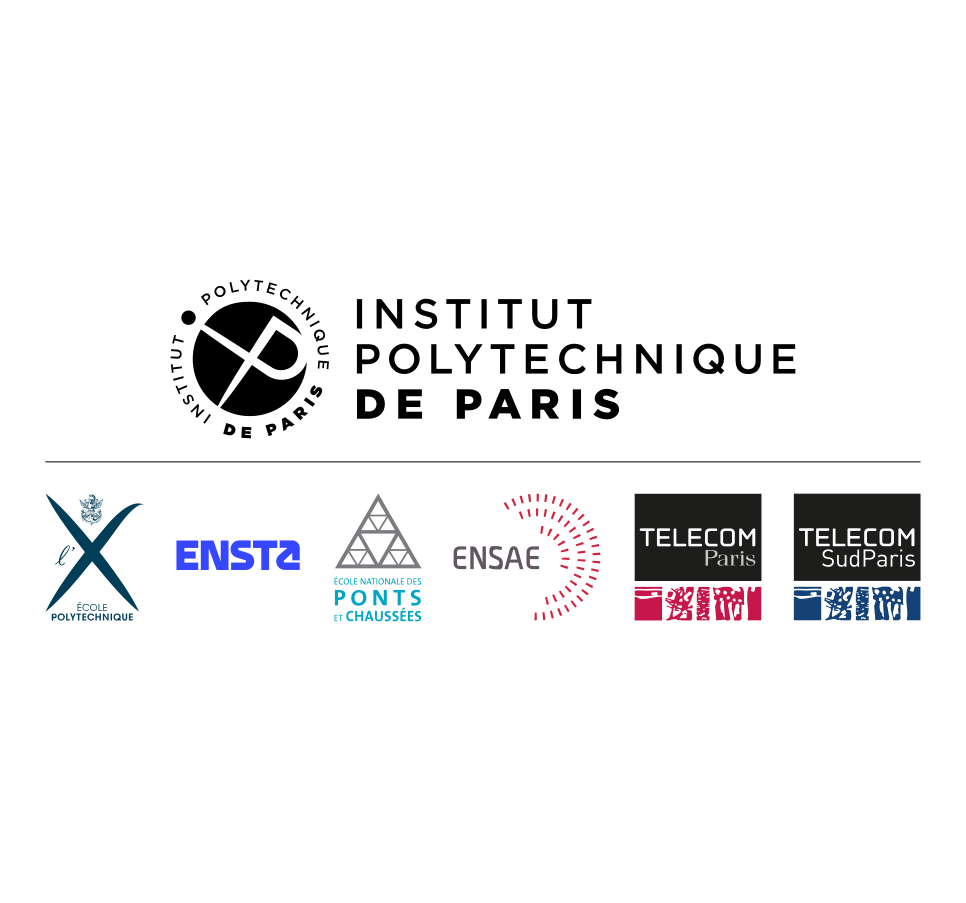
\includegraphics[width=0.5\textwidth]{logo-ipparis.png} % Logo (converted from SVG)

\vspace{-1em} % Pull the rule closer to the logo

\rule{\linewidth}{1pt} % Horizontal rule

\bigskip\bigskip % Vertical whitespace

%----------------------------------------------------------------------------------------
%	YOUR NAME AND CONTACT INFORMATION
%----------------------------------------------------------------------------------------

\hfill
\begin{tabular}{l @{}}
	\today \bigskip\\ % Date
	Augustin Bresset \\
	36 Rue des Gravilliers, 75003 \\ % Address
	Phone: +33 6 51 09 26 88 \\
	Email: augustin.bresset@ip-paris.fr
\end{tabular}

\bigskip % Vertical whitespace

%----------------------------------------------------------------------------------------
%	ADDRESSEE AND GREETING
%----------------------------------------------------------------------------------------

\begin{tabular}{@{} l}
    Dr.\ Emmanuel De Bézenac \\
    Research Scientist, ARCHES Team \\
    Inria Paris \\
    2 Rue Simone Iff \\
    75012 Paris, France
\end{tabular}

\bigskip % Vertical whitespace

Dear Dr.\ De Bézenac,

\bigskip % Vertical whitespace

%----------------------------------------------------------------------------------------
%	LETTER CONTENT
%----------------------------------------------------------------------------------------

I am writing to express my interest in the Research Internship (M2) titled “Building efficient generative models for weather forecasting” within the ARCHES team at Inria Paris. I am currently completing a double degree between the Master of Data Science at École Polytechnique and the engineering curriculum at Télécom SudParis, and I am looking for a research internship starting in April 2026 as part of my master's thesis. I learned about this position on Inria’s recruitment website and was immediately drawn to its scientific focus and to the opportunity to work under the supervision of Dr. Emmanuel De Bézenac.

My academic background and research interests are closely aligned with the objectives of this internship. Through advanced courses in convex analysis, stochastic approximation, Markov-chain methods, hidden Markov models, deep learning, reinforcement learning, and online learning, I have built a strong foundation in the mathematics and theory underlying modern machine learning. In parallel, my coursework and personal projects have cultivated a deep interest in generative modeling—particularly diffusion models, flow matching, and neural architectures capable of capturing complex dynamics.

My previous research internship at ENSTA Paris strengthened my ability to conduct exploratory scientific work, where I developed a unified Python framework for heterogeneous robotic datasets and worked with PyTorch and ROS to preprocess and evaluate models in a research environment. Additionally, my software engineering internship at Rubicon (Bangkok) demonstrates my capacity to develop robust systems autonomously and handle large-scale data pipelines. These experiences, combined with my long-term goal of pursuing a PhD in machine learning and optimization, motivate my wish to contribute to the development of next-generation generative models for atmospheric prediction. I am particularly interested in the multiscale and spectral aspects highlighted in the internship description, and in understanding how model architecture influences physical fidelity and stability. A detailed summary of my technical skills and experience can be found in the attached CV.

I would be very happy to further discuss my application and the ways in which I could contribute to the ARCHES team. I am fully available for an interview at your convenience, onsite or remotely, and can be reached at +33 6 51 09 26 88 or by email at augustin.bresset@ip-paris.fr

\bigskip % Vertical whitespace

Sincerely yours,

\includegraphics[height = 1cm]{signature_bw.jpg}

\vspace{25pt} % Vertical whitespace

Augustin Bresset

\end{document}
